\chapter{Running Kubernetes}

I~will run Kubernetes on 3 testing machines. First decision I~have to make is which operating system I~will use. Since almost all machines in Seznam.cz data centres are running Debian I~will use it as well on my testing cluster and I~will install its newest stable version Jessie. There are Linux distributions made especially for Kubernetes like Fedora Atomic \cite{fedora-atomic}, but as our administrators have many years of experience with Debian, it will be better to use it instead of changing architecture to cloud and changing Linux distribution at the same time.

Another decision that has to be make is about networking.

\section{Networking in Kubernetes}

Kubernetes assumes that pods can communicate with other pods, regardless of which host they land on. They give every pod its own IP address so I~do not need to explicitly create links between pods. This creates a clean, backwards-compatible model where pods can be treated much like VMs or physical hosts from the perspective of port allocation, naming, service discovery, load balancing, application configuration, and migration. \cite{kubernetesdoc}

\subsection{Docker model}
Before discussing the Kubernetes approach to networking, it is worthwhile to review the ``normal" way that networking works with Docker. By default, Docker uses host-private networking. It creates a virtual bridge, called docker0 by default, and allocates a subnet from one of the private address blocks defined in RFC1918 \cite{rfc1918} for that bridge. For each container that Docker creates, it allocates a virtual Ethernet device (called veth) which is attached to the bridge. The veth is mapped to appear as eth0 in the container, using Linux namespaces. The in-container eth0 interface is given an IP address from the bridge’s address range.

The result is that Docker containers can talk to other containers only if they are on the same machine (and thus the same virtual bridge). Containers on different machines cannot reach each other –- in fact they may end up with the exact same network ranges and IP addresses.

In order for Docker containers to communicate across nodes, they must be allocated ports on the machine’s own IP address, which are then forwarded or proxied to the containers. This obviously means that containers must either coordinate which ports they use very carefully or else be allocated ports dynamically. \cite{kubernetes-networking}

\subsection{Kubernetes model} 
Coordinating ports across multiple developers is very difficult to do at scale and exposes users to cluster-level issues outside of their control. Dynamic port allocation brings a lot of complications to the system – every application has to take ports as flags, the API servers have to know how to insert dynamic port numbers into configuration blocks, services have to know how to find each other, etc. Rather than deal with this, Kubernetes takes a different approach.

Kubernetes imposes the following fundamental requirements on any networking implementation (barring any intentional network segmentation policies):

\begin{itemize}
\item	all containers can communicate with all other containers without NAT
\item	all nodes can communicate with all containers (and vice-versa) without NAT
\item	the IP that a container sees itself as is the same IP that others see it as
\end{itemize}

In reality, Kubernetes applies IP addresses at the pod scope -- containers within a pod share their network namespaces -- including their IP address. This means that containers within a pod can all reach each other’s ports on localhost.

This networking mode is implemented in many different ways. The basic one and the one which is mentioned in documentation of Kubernetes is flannel. \cite{kubernetes-networking}

\subsubsection{Flannel}
Flannel is a virtual network that gives each host a subnet for use with container runtimes.

Platforms like Google's Kubernetes assume that each container (pod) has a unique, routable IP inside the cluster. The advantage of this model is that it reduces the complexity of doing port mapping.

Flannel runs an agent, flanneld, on each host and is responsible for allocating a subnet lease out of a preconfigured address space. Flannel uses etcd to store the network configuration, allocated subnets, and auxiliary data (such as hosts' IP addresses). The forwarding of packets is achieved using one of several strategies that are known as backends. The simplest backend is UDP and uses a TUN device to encapsulate every IP fragment in a UDP packet, forming an overlay network. The following diagram \ref{fig:flannel} demonstrates the path a packet takes as it traverses the overlay network. \cite{flannel}
                              
\begin{figure}[htb]\centering
  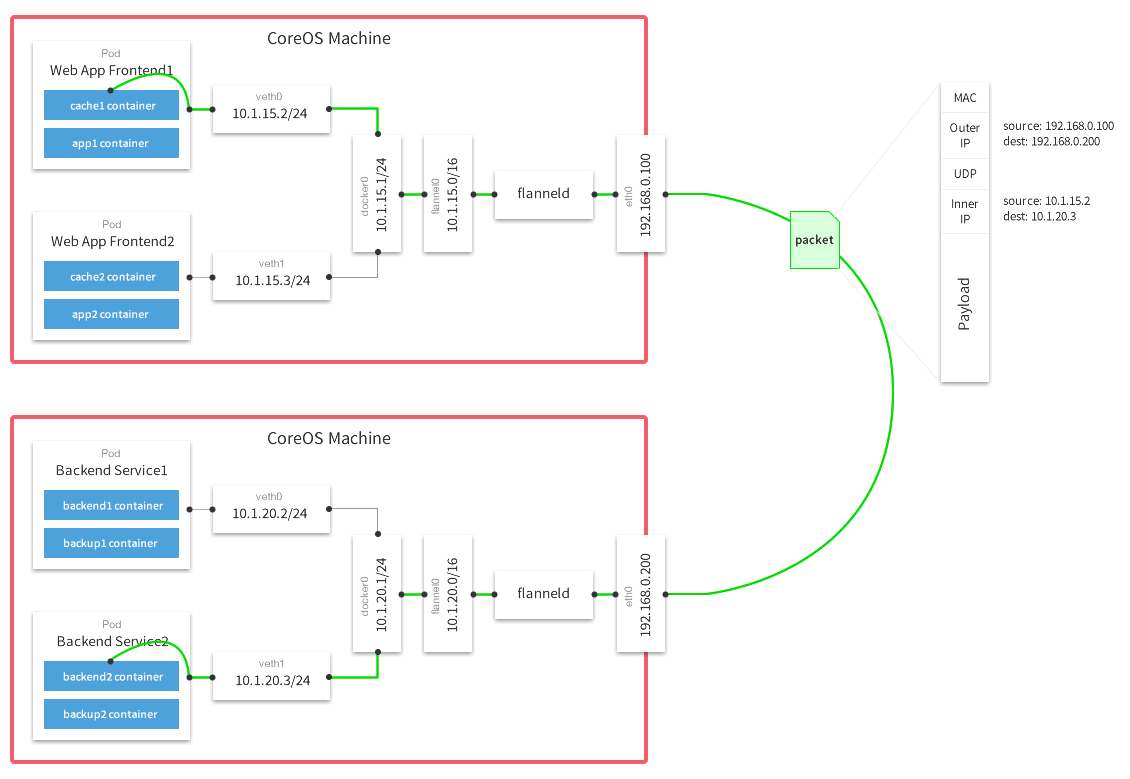
\includegraphics[width=1\textwidth]{images/flannel.png}
  \caption
    [The path of a packet in flannel network]
    {The path of a packet in flannel network \cite{flannel}}
  \label{fig:flannel}
\end{figure}

Flannel is simple to start up but there can be some overhead expected. It is needed to test how big overhead it will be. Another big disadvantage of flannel is that it is not multitenant and so there is no way how to define any rules who can communicate with whom and who can’t. In practice that means everyone sees everyone. For introducing cloud at Seznam.cz it can be sufficient but in the future this needs to be solved more properly so there can be policies defining restricted access to sensitive services.

\subsubsection{Calico}

Next networking option is Calico. Calico provides a highly scalable networking solution for connecting data center workloads (containers, VMs, or bare metal). It is based on the same scalable IP networking principles as the internet: providing connectivity using a pure Layer 3 approach. Calico can be deployed without encapsulation or overlays to provide high performance at massive scales.

When using Calico networking in containerized environments, each container gets its own IP address and fine grain security policy. A~calico-node service runs on each node which handles all of the necessary IP routing, installation of policy rules, and distribution of routes across the cluster of nodes.  \cite{calico}

Calico has even a section dedicated for Kubernetes in their manual \cite{calico-kubernetes}. They state that thanks to that there is no overlay, Calico will be faster than technologies that use overlay, such as flannel. Calico is using the Bird \cite{bird} system for route distribution around the network.

\subsubsection{OpenContrail} 

On the meeting with company tcp cloud \cite{tcpcloud} technology OpenContrail was discussed \cite{tcpcloud-opencontrail}. OpenContrail is a network virtualization platform for the cloud. It has been designed with scale out in mind  \cite{opencontrail}. OpenContrail is a representative of SDN (software defined networking) and it offers to define custom policies of containers communication thanks to label system in Kubernetes. It will be worth it to examine whether this technology fits for Seznam.cz needs and environment.

\section{Starting cluster}
From listed options of network management I~decided to start with a simple one: the flannel. This thesis should create a proof of concept that it is possible to maintain Kubernetes in Seznam.cz. I~want to create a testing application and an example Kubernetes cluster where I~solve all potential problem described in the previous chapter and then I~give this to our administrators who may test it further as they want to.

Running flannel containers needs privileged permissions but user defined pods and their containers should not ever have such permissions. So the best way how to achieve this behaviour is to start two separate Docker daemons where one will allow to create privileged containers and the second one won’t.

Starting Docker on Seznam.cz corporate machines brought a couple of problems that must be solved first. From Seznam.cz system preinstaller in \lstinline{/etc/network/interfaces} all routes to private IPs are routed via eth0 interface which cases that Docker could not find and private IP range free for its purposes. This can be simply solved by freeing an IP range and restarting network service together with Docker daemon.

Next issue that occured was a little bit tougher. In the Docker log I~found that no chain exists for an iptables rule which Docker wants to set. After consulting this problem with my team leader it proved to be caused by missing kernel modul \lstinline{xt_conntrack}. After adding this module to kernel Docker daemon finally started.

In the Docker log I~also found a warning that cgroup memory is not allowed and that could possibly cause Kubernetes to not work properly with pod memory limitation. I~added the following line to the \lstinline{/etc/default/grub} file and updated grub.
\begin{lstlisting}[language=bash]
  GRUB_CMDLINE_LINUX="cgroup_enable=memory swapaccount=1"
\end{lstlisting}

With the Docker daemon running I~could start Kubernetes. As was shown in the \nameref{chapter:kubernetes-basic-concepts} chapter, the master node has to have API server, scheduler, proxy, kubelet, controller-manager and flannel running in a separate Docker daemon.

The first step is to create a bootstrapped daemon. The second is to run etcd. I~used \lstinline{gcr.io/google_containers/etcd-amd64} image. The third is to setup flannel. I~also used a prebuilt image, this time \lstinline{quay.io/coreos/flannel}. Finally the last step is to start kubelet. Kubernetes offers prebuilt Docker image with all its components included called \lstinline{gcr.io/google_containers/hyperkube-amd64}. From the hyperkube image the kubelet is called and in configuration of the kubelet there is a set of static pods that should be created. The hyperkube firstly creates those pods and then starts the kubelet. Those pods are the scheduler, the API server, the controller-manager and the kube-proxy.

I~have prepared a script where this whole configuration is scripted and which may be called with the following single line: \lstinline{./kube.sh start-master} You can also specify which components should be started.

Now the worker has to be set. The configuration is similar only there is not so many components to run. The first step is also to create a bootstrapped daemon, then the flannel and the kubelet are started, respectively. The kubelet is configured to run only kube-proxy.

Now adding a new worker node to the cluster is very simple. Install the system, fix problems described earlier and then upload a script and run .\lstinline{/kube.sh start-worker}. This system may be automated with ansible \cite{ansible} for example but this is a task for our administrators.

Also there are other possibilities how to run this Kubernetes model. The kubelet can be installed on bare-metal and not be dockerized and the same applies to the flannel. But it really is just a matter of personal preferences.

The cluster is now fully functional and pods may start to be distributed.

\begin{figure}[htb]\centering
  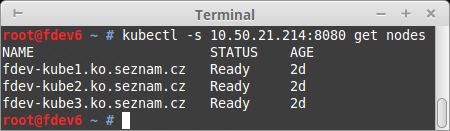
\includegraphics[width=0.95\textwidth]{images/kubectl_get_nodes.png}
  \caption
    {Screenshot of \lstinline{kubectl get nodes} output}
  \label{fig:kubectl-get-nodes}
\end{figure}

